%%%%%%%%%%%%%%%%%%%%%%%%%%%%%%%%%%%%%%%%%%%%%%%%%%%%%%%%%%%%%%%%%%%
%                                                                 %
%                            CHAPTER ONE                          %
%                                                                 %
%%%%%%%%%%%%%%%%%%%%%%%%%%%%%%%%%%%%%%%%%%%%%%%%%%%%%%%%%%%%%%%%%%%

\chapter{INTRODUCTION} \label{sec:introduction}

A sketch is a rough or unfinished drawing that represents the essential features without all the details. However, the absence of detail in a sketch does not make it less significant than a finished drawing. Sketches allow designers to express their ideas to others in a quick manner, without committing themselves fully. The agile nature of sketches also allow designers to rapidly prototype many ideas while receiving feedback on their work. With this combination of traits, sketching becomes the ideal method of exploring and refining new ideas. \\

The purpose of sketching is twofold: to convey ideas to others and to explore new designs. It is simple to imagine a concept in your head for yourself, it is a completely different challenge to communicate that concept to another person. The ability to effectively communicate your ideas to a client or peers is invaluable in saving time and stimulates productive conversation on the design itself. Sketching is helpful in getting across basic elements about an idea without spending too much time on smaller details. Due to the speed at which sketches can be produced, a designer can afford to explore new, untested ideas. The designer can then aggregate the best qualities, or learn what to avoid in future designs. The two purposes of sketching are closely related and can used to build off one another.

\section{Architectural Drawings and Sketches}
Architects create many sketches and drawings when designing a structure, each with varying degrees of detail. Each image serves its own purpose and has its place within the architectural design process. Sketches are appropriate earlier in the design process when an image's main purpose is to express the architect's design and meet the owner's goals and expectations, while drafts are more appropriate later in the process when contractors need to approximate cost and physically construct the building. Typically, as the process progresses, the level of detail increases. As more details are finalized, and less pieces of the design are left to interpretation.

\subsection{Sketches}

\begin{figure}[ht]
\centering
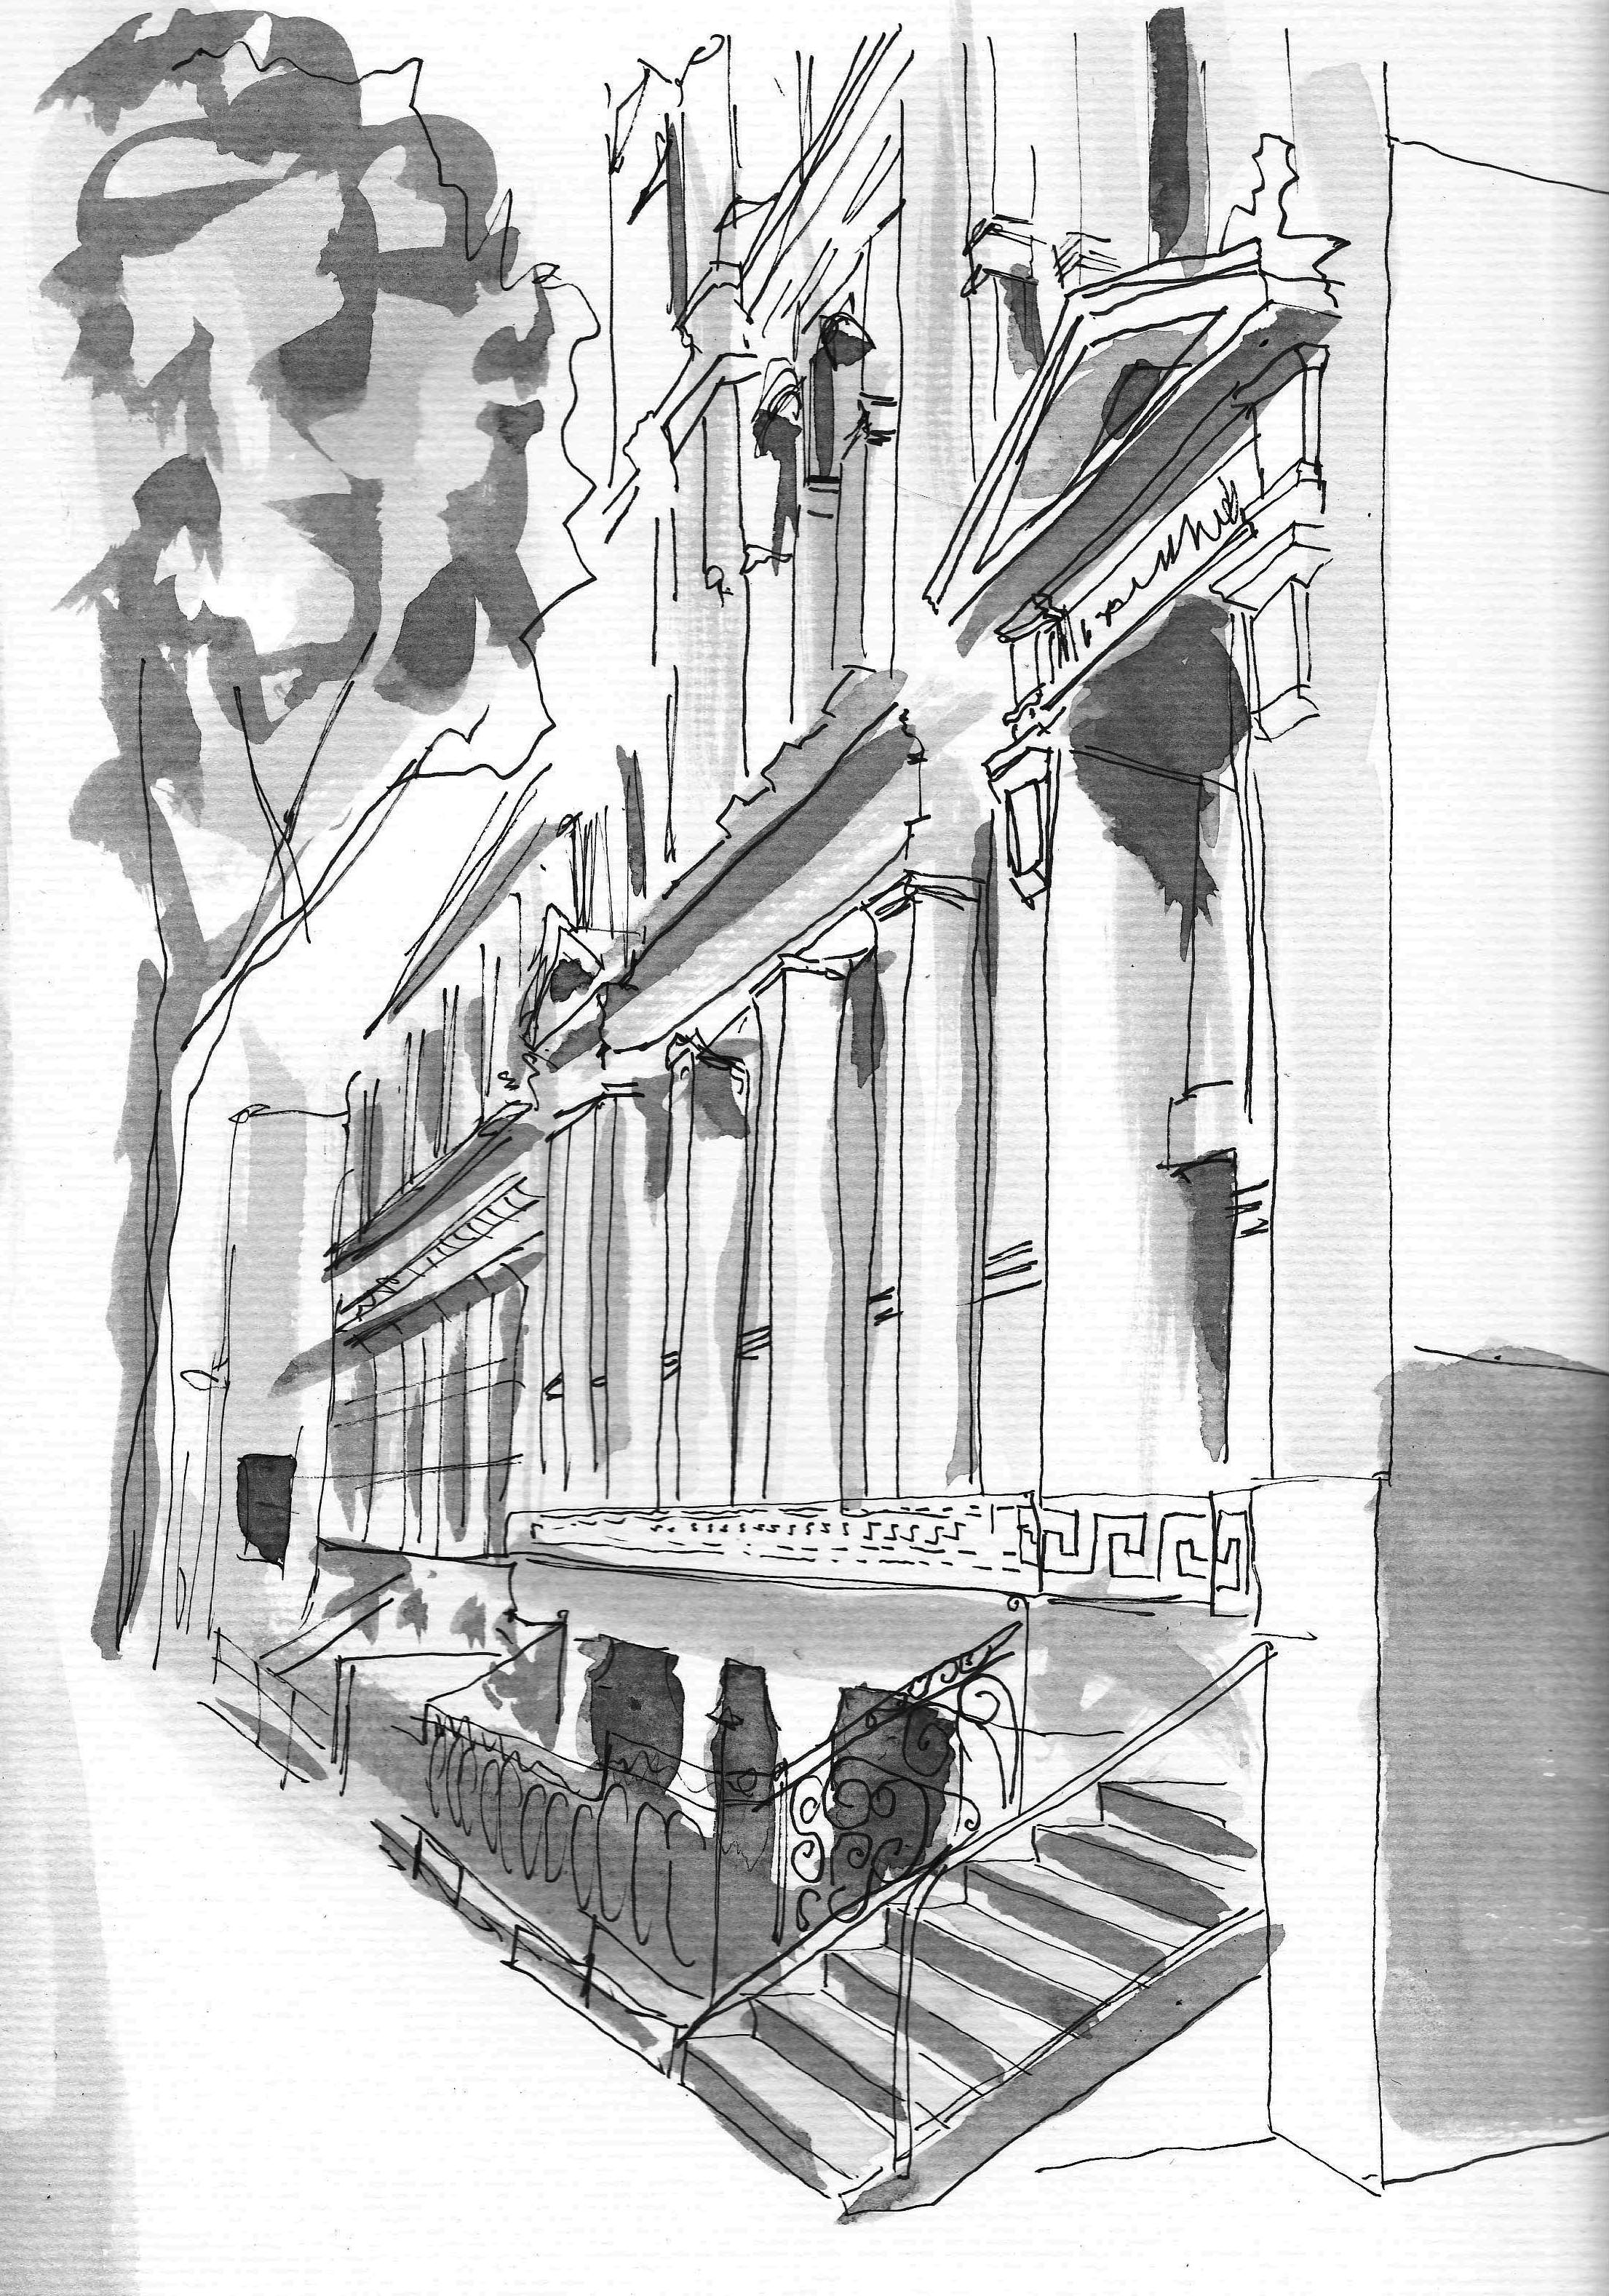
\includegraphics[width=.6\textwidth]{quicksketch}
\caption[Example of a quick architectural sketch.]{A quick sketch depicting the front view of the Lombard Building on Queen Street, Melbourne. Sketched by Aushist, used under GNU Free Documentation License \cite{quicksketch}.}
\label{fig:quicksketch}
\end{figure}

Sketches are among the most basic drawings created by architects. Their simplicity in creation and design allow for quick modification of ideas and ease of understanding of general concepts. No initial sketch needs to have correct scale or the dimension numbers, as long as the ideas of the designer reach his or her intended audience. Without too much detail, audience can focus on the key details the designer has purposefully chosen to include in the sketch. A sketch is the perfect vehicle for rapid prototyping and design analysis, without the accuracy and time commitment required for producing a draft. \\

\begin{figure}[ht]
\centering
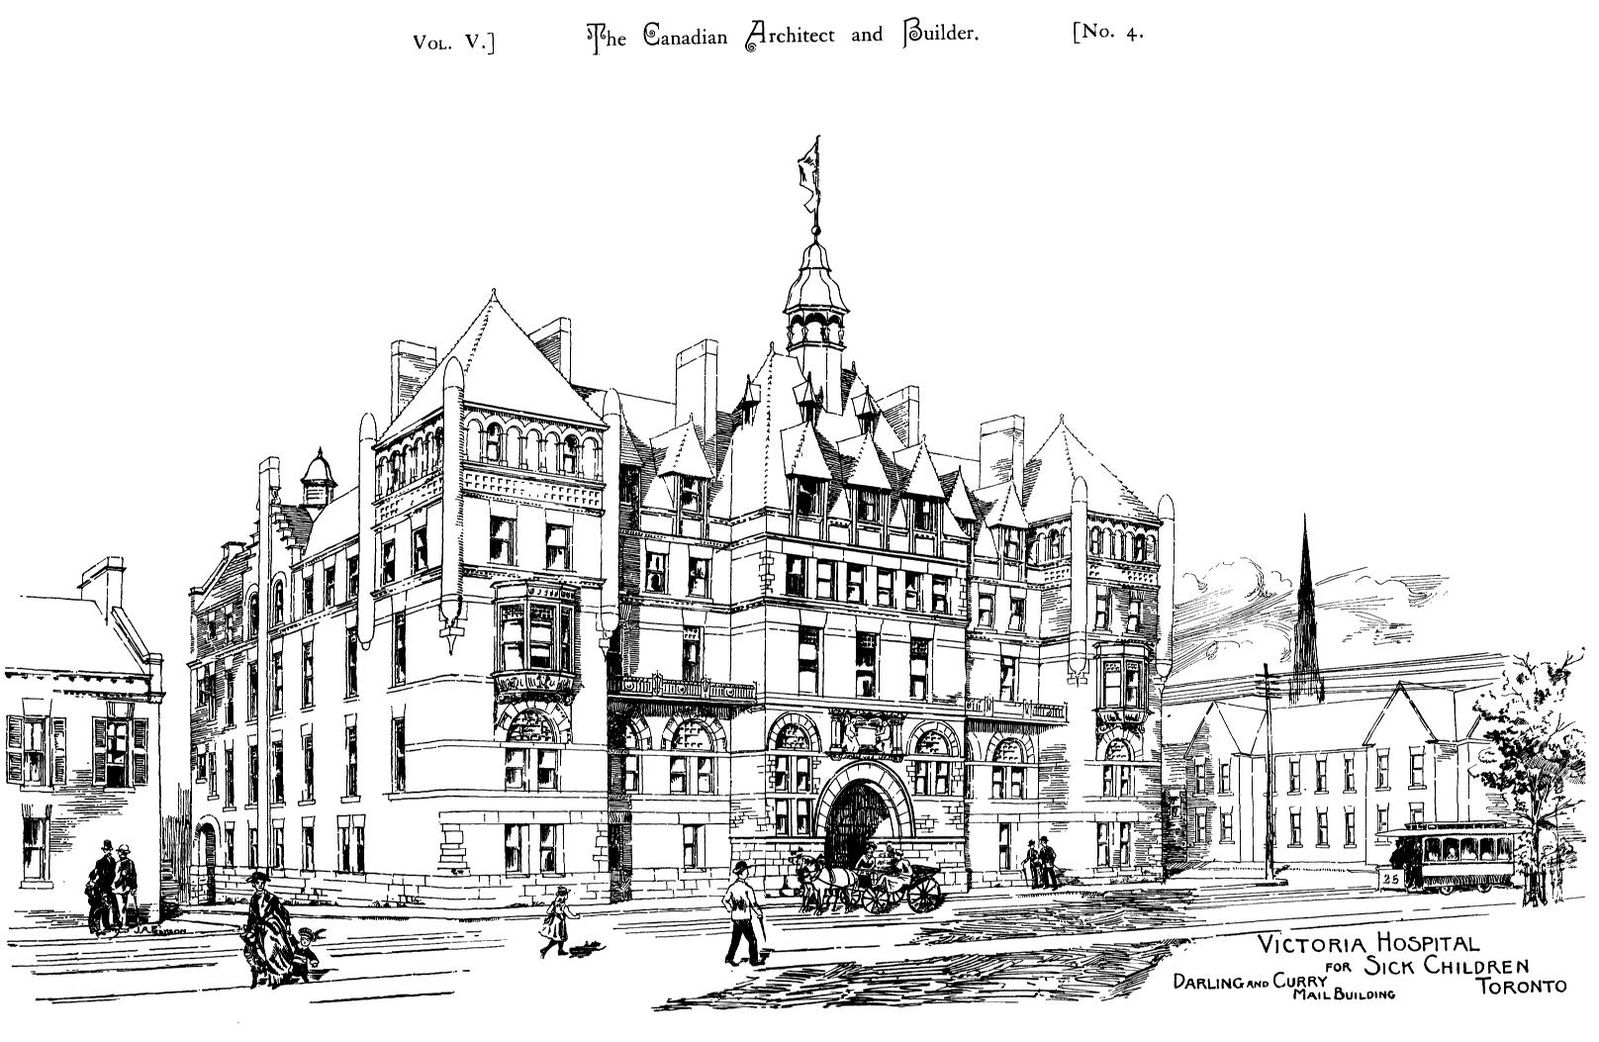
\includegraphics[width=\textwidth]{archsketch}
\caption[Example of an architectural sketch - elevation view]{An architectural sketch of the elevation view depicting the Victoria Hospital for Sick Children. Drawn by Darling and Curry work is in public domain \cite{hospital}.}
\label{fig:archsketch}
\end{figure}

Depending on what needs to be shown, architects can sketch their design from many different angles \cite{drafting_and_design}. A floor plan is the fundamental view for a building. It displays the layout of the building at a certain elevation, showing details on a floor by floor basis, as shown in Figure \ref{fig:topdownsketch}. For a side view the interior, an architect can construct a cross section view. A cross section view is an image of the building from the side, cut by a plane. It shows the relationship between different floors, and how they are layered on top of each other. If a client wants to see how a building appears from the outside, the architect can present an elevation view, such as the one illustrated in Figure \ref{fig:archsketch}. An elevation view is a flat view from the outside of building at a certain height, showing one face of the structure. Since most buildings are not the same at all angles, elevation views from multiple angles may be constructed. One particular angle is an isometric angle, which is a view where the angles between the projections of all axes are equivalent. As shown in the left image in Figure 1.1, an isometric view displays the outside only, and shows the connections between outside elements. To show the context around where a building is located, a site plan is created. It is an overhead view, similar to a floor plan, but it displays the whole property instead of one building. When designing a building, an architect will create most, if not all, of these views to present to the owner so he/she can accurately understand the architect's ideas.

\subsection{Drafting}

Before an architect's design can become a building, architectural drafts of the design need to be created. Drafts are extremely high detail drawings depicting dimensions, structure, and layout of a building \cite{drafting_and_design}. There exists drafts of many aspects of the building, such as electrical, plumbing, and structural. These drafts help guide the contractors to construct the building according to the design and specifications set by the architect and owner. Before the existence of computer-aided drafting (CAD) software, drafts were created meticulously by hand. Drafts were checked by many people; small mistakes could have massive consequences on the structure of a building. 

\begin{figure}[ht]
\centering
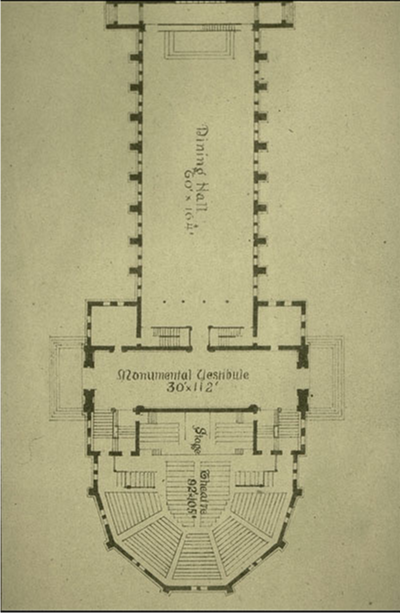
\includegraphics[width=.8\textwidth]{rotated}
\caption[Example of a hand drawn architectural sketch - floorplan]{A hand drawn architectural floorplan of Memorial Hall (Harvard University). Author unknown, work is in public domain \cite{harvard}.}
\label{fig:topdownsketch}
\end{figure}

% AutoCAD SolidWorks NX

With the rise of computing power through the 1970's and 1980's, so too did the benefits of switching over to computer-aided drafting (CAD). CAD software drastically increased the quality of designs produced, improved communication between architects and engineers, and boosted productivity \cite{cad}. CAD software creates more accurate drafts, without object scales needing to be manually verified. Control over information about structure, electricity, plumbing and much more are all organized and displayable on a whim. Editing the project is no longer as tedious; objects can be deleted, copied, rotated, and scaled, with few button clicks. The benefits of using CAD software are immense, and its prevalence in fields such as architecture and engineering reflects that.

\begin{figure}[ht]
\centering
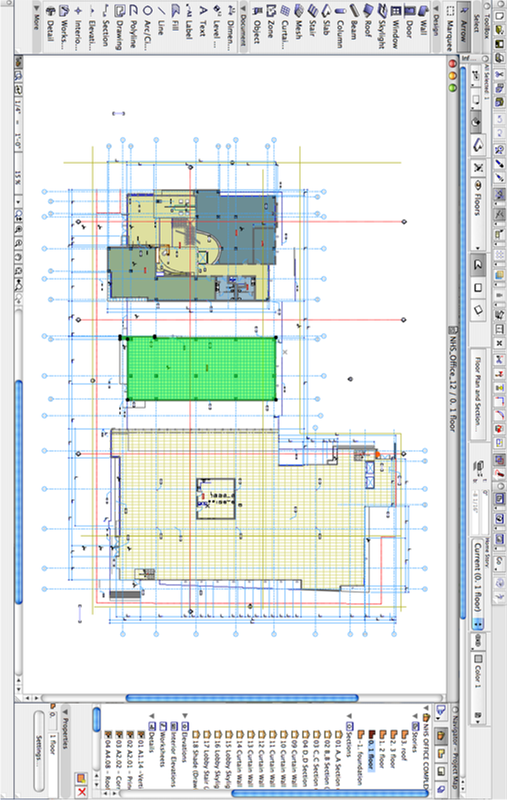
\includegraphics[width=.75\textwidth]{cadrotate}
\caption[Example of a room designed using CAD software]{An example floor plan created using ArchiCAD \cite{archicad}. Created by Martinremco, work is used under Creative Commons \cite{cad1}.}
\label{fig:cad1}
\end{figure}

The sheer strength of the tools available with CAD software dwarfs the power of a person with pencil and paper, and the drawings produced by both mirrors that imbalance. To produce a draft with the same quality, a hand drawn model would take a great deal more time and effort compared to one created with software. Using tools such as AutoCAD \cite{autocad}, ArchiCAD \cite{archicad}, and NX \cite{nx}, designers have more power than ever. Figure \ref{fig:cad1} illustrates one example of a design using ArchiCAD. However, using CAD software is not without its downsides. Compared to drawing on paper, a large amount of training or familiarity with the program is required to proficiently create drafts. Improper use of software can be a hindrance when designing, making other tasks more difficult. Since software is constantly changing, there continues to be more learning required, especially with large updates or feature changes. Despite all the drawbacks, CAD software continues to be a leading choice for many architects and engineers.

\section{The Architectural Design Process}

Architects often follow a five step process from design to completion of a building. The five phases are: schematic design, design development, construction documents, bid or negotiation, and construction administration \cite{bestpractices}. During the schematic design phase, the architect and client work together to determine the goals and needs of the project. The architect creates drawings and documents to accurately show their concept to the owner. He or she also researches zoning and jurisdictional restrictions to present to the client. At the end of this phase, the architect will produce a final schematic design that will be the basis for cost, design, and development. Next, during the design development phase, details for multiple elements of the building are finalized, including windows, walls, and doors. Structural details such as plumbing and electrical are also settled upon. After, the construction documents are created with the information from the design development phase. A schematic design is created with even greater detail for contractors to pricing and bidding. Afterwards, bids and negotiation begin for the construction of the building. The owner and architect will review bids and select a contractor to construct the building. Finally, the construction begins on the project. Though out construction of the building, The architect will continue to help the contractor build the project as specified in the documents created during the construction documents phase. \\

% We focus primarily on the the earliest portion of the schematic design phase. 

Design plays a crucial role in the architectural design process. Each phase builds off the work done in previous stages, so the design done during the schematic design phase is the foundation for the rest of the project. Our focus in this thesis work is to improve the schematic design phase of the architectural design process. We hope to facilitate more efficient exploration of new ideas, as well as a smoother transition into the next phase.

\section{Benefits of Sketching in Design}

% Sketching typically occurs during the infancy of any project, whether it be a piece of artwork or schematics for a building. This phase is often called the design phase. The ideas and thoughts manifested during this phase are the foundation for what is created in later phases.

% Design, or inception of an idea, is often the first step in creating a successful building. Good design is a combination of many features: usefulness, aesthetics, and so on.

The term "design" can be used to describe many different actions or creations across many fields. References can be drawn to graphic design in art, engineering design, the design of computer code, design of production processes, even the process of design itself \cite{howdesignersthink}. In some cases, design can be construction of the object itself, such as a piece of artwork. In essence, design is the manifestation of an idea into a plan or drawing to accomplish some task or goal. For example, when tasked with designing a website, I sketched out some designs before constructing anything. The results are show in Figure \ref{fig:websitesketch}. Being able to design well means merging individual components together cohesively to accomplish some objective. Achieving the goal in the most efficient and elegant way possible is the ambition of all designers. \\

\begin{figure}[ht]
\centering
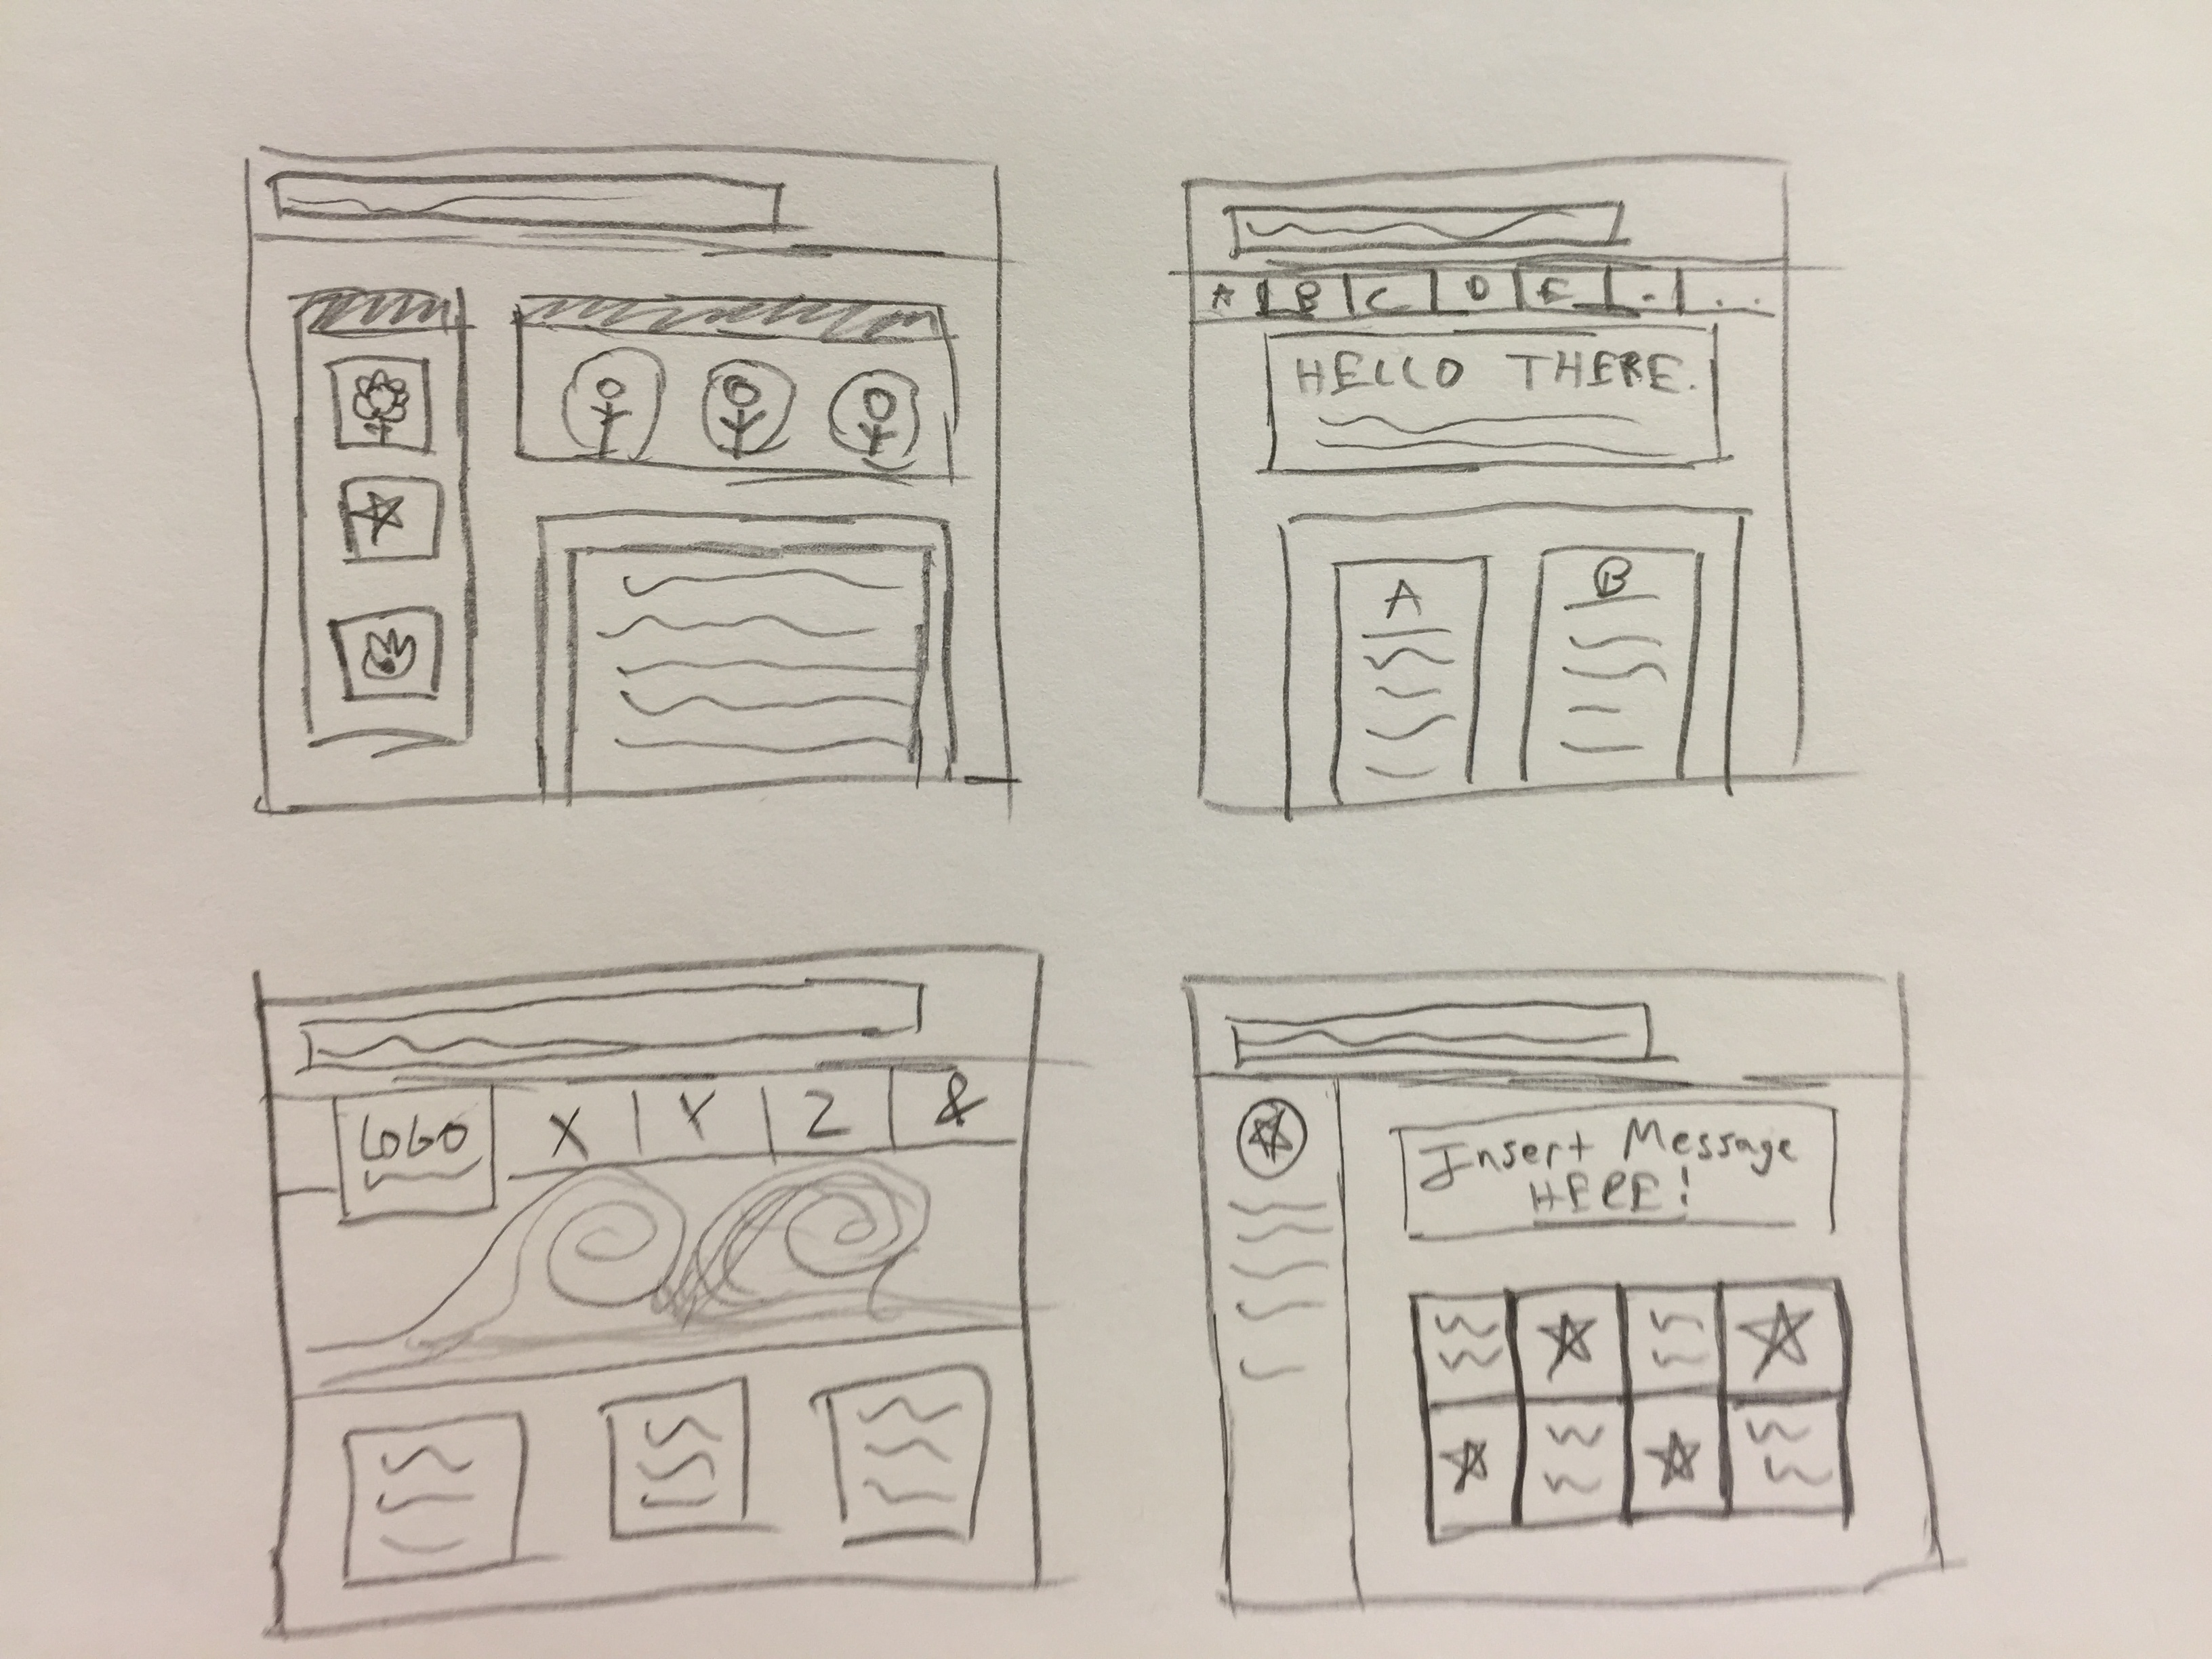
\includegraphics[width=\textwidth]{webdrawing}
\caption[Design sketch examples drawn when tasked with designing a website.]{Sketches drawn when tasked with designing a website.}
\label{fig:websitesketch}
\end{figure}

There are many benefits to sketching ideas when designing. Throughout the design process, sketching is invaluable for communicating ideas \cite{ullmanwood1990}. Sketching is a self reflective process, and allows for the designer to efficiently map out their thoughts in a manner that makes more sense \cite{howdesignersthink}. Seeing, moving, improving their designs helps users increase their design proficiency \cite{schon2004}. Song and Agogino \cite{song2004} observed that there was a positive correlation between usage of sketches and the user's design outcome. The process of making sketches to solve problems also induces a 'design reasoning' that increases visual thinking and puzzle solving \cite{dialects}. Studies have shown that not only did sketching allow the designer to think more creatively, it also stimulated the clients those designers were working for \cite{Schutze2003}.  When sketching, designers more often than not changed their original ideas and formed new ones, while those who used a drawing program were more limited in what they created. There have been positive correlations found between number of designs and the outcome, as observed by Yang \cite{yang2009}. In the early design process, self made sketches increased the quality of solutions proposed, as well as having an overall positive impact on the final product. Users who had the opportunity to sketch their ideas in the design phase found the problems to be significantly easier and this solution quality increased \cite{Schutze2003}. These user thought the solution was much more intuitive and were able to logically progress through a solution more quickly for the problem at hand. \\

A similar process can be used in architectural sketching implementations. The ability to sketch out ideas can have a positive impact on the overall end product. The importance of sketching to an architect cannot be understated. Sketching as a tool has been observed to be valuable when used for creative tasks \cite{Schutze2003}. Utilizing the creative power of sketching, we aim to create an interface that improves the design potential of all its users.

\section{Thesis Outline and Contributions}

This thesis is motivated by the creation of the Online Architectural Sketching Interface for Simulations (OASIS) \cite{oasis2016}. There was a desire to create a more novel, cohesive, and intuitive way to design models. The previous iteration of OASIS utilized a drag-and-drop user interface for creating designs. To improve the system, imitating how architects design buildings seemed like the most logical option. Architects design buildings first on pencil and paper, then transition to a CAD program to add further detail. By accepting inputs as strokes, we hope to give the user freedom and flexibility that was not available in the previous iteration. \\

The first step in creating a solution that met our goals was to create a process that accepted user input in the form of strokes. Chapter 2 outlines some of the work leading up to the creation of this sketching interface. Next, chapter 3 explains the pipeline of OASIS, how this work modifies and improves previous features, and basic elements of the interface. Chapters 4 details how the system uses the simple strokes input by the user to create a design that matches the user's intentions. Chapter 5 includes a small informal pilot study on the usage of the current interface against the previous one. Finally, chapter 6 concludes with closing remarks and potential directions for further improvements and research.